\section{Theoretischer Hintergrund des Versuches}
\label{sec:Theorie}
\subsection{Energieniveaus der Rubidiumisotope}
Mit einer Ordungszahl von $Z=\num{37}$ befindet sich Rubidium in der 
fünften Periode der ersten Gruppe im Periodensystem und ist somit ein
Alkalimetall. Die Elektronenkonfiguration dieser wird nur durch 
das einzige Valenzelktron bestimmt, da alle darunterliegenden Schalen
vollständig gefüllt sind. Aus der Elektronenkonfiguration 
$\text{[Kr]}5\text{s}^1$ folgen nach den Hundeschen Regeln
\begin{equation*}
    \ket{n,L,M_L}=\ket{5,0,0},
\end{equation*}
wobei $n$ die Hauptquantenzahl,$L$ die Drehimpulsquantenzahl
und $M_L$ die magnetische Quantenzahlen bezeichnet. Die 
Hauptquantenzahl $n$ ist in niedrigster Ordnung mit $L\in [0,n-1]$ und 
$M_L\in[-L,L]$ entartet. 

\subsubsection{Feinstrukturaufspaltung}
Unter Berücksichtigung des Elektronenspins
wird die Entartung in $L$ gebrochen, da jedem Gesamtdrehimpuls 
$\vec{J}=\vec{L}+\vec{S}$ von 
$|L-S|$ bis $|L+S|$ eine andere Energie zugeordnet wird. Diese 
Korrektur wird Spin-Bahn-Kopplung genannt. Die magnetische Quantenzahl
$M_J$ ist nun dem Gesamtdrehimpuls zugehörig. Sie bleibt jedoch mit 
$M_J\in[-J,J]$ entartet. Die durch die Aufspaltung entstehende Struktur
der Energieniveaus wird Feinstruktur genannt. 

\subsubsection{Hyperfeinstrukturaufspalung}
Eine höhere Korrektur bildet die Hyperfeinstruktur. Bei dieser wird 
die Wechselwirkung des Kernspins $I$ mit dem Gesamtdrehimpuls $J$ der
Elektronenhülle betrachtet. Analog zur Feinstruktur kann der Gesamtdrehimpuls
$\vec{F}=vec{J}+\vec{I}$ Werte von $|J-I|$ bis $|J+I|$ annehmen. 
Die Entartung der zugehörigen magnetischen Quantenzahl $M_F$ bleibt
abermals unverändert. Die Entartung in $F$ jedoch wird aufgehoben. 
Die beiden betrachteten Isotope $\ce{^{85}Rb}$ und $\ce{^{87}Rb}$
unterscheiden sich in dem Kernspin
\begin{align*}
    I_{^{85}Rb}&=5/2\\
    I_{^{87}Rb}&=3/2
\end{align*}
und dementsprechend auch im Gesamtdrehimpuls $F$.

\subsubsection{Der Zeeman-Effekt}
Aus Symmetrieüberlegungen folgt, dass die Entartung der magnetischen 
Quantenzahl durch die Brechung der Rotationssymmetrie aufgehoben wird.
Beim Zeeman Effekt geschieht dies durch ein magentisches Feld. 
Die Energieniveaus werden dabei mit einer Differenz von 
\begin{equation}
    \Delta E_Z=g_F\mu_B M_F B
\end{equation}
aufgespalten, wobei $g_F$ der Landé-Faktor, $\mu_B$ das Bohrsche Magneton
und $B$ die Flussdichte des angelegten Magentfeldes ist. Der Landé-Faktor
ist gegeben durch 
\begin{equation*}
    g_F=g_J\frac{F(F+1)+J(J+1)-I(I+1)}{2F(F+1)}
\end{equation*}
mit 
\begin{equation*}
    g_J=1+\frac{J(J+1)+S(S+1)-L(L+1)}{2J(J+1)}.
\end{equation*}

\noindent
In Abbildung \ref{fig:niveaus} ist sind die Aufspaltungen der verschiedenen
Korrekturen für $\ce{^{85}Rb}$ qualitativ dargestellt.
\begin{figure}[H]
    \centering
    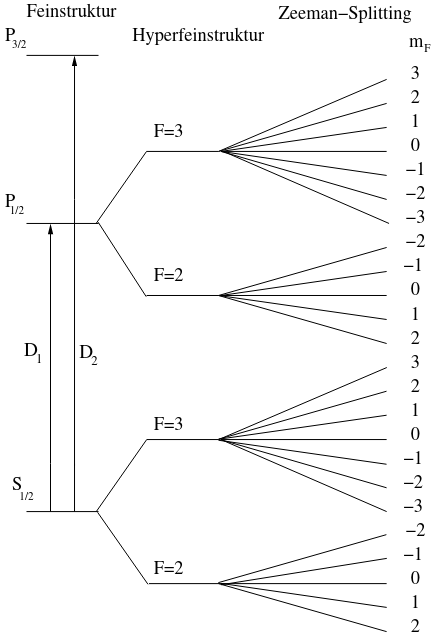
\includegraphics[scale= 0.4]{pictures/Niveaus.png}
    \caption{Schematische Darstellung verschiedene Energieaufspaltungen für $\ce{^{85}Rb}$ \cite{OptischesPumpen}.}
    \label{fig:niveaus}
\end{figure}

\subsubsection{Der quadratische Zeeman Effekt}
Der anormale Zeeman Effekt wird mathematisch durch einen Stör-Hamiltonian
zusätzlich zu der Feinstruktur beschrieben. Wird der Einfluss des 
Magnetfeldes größer als der der Feinstruktur, wird die Feinstruktur
als Störung zum Magnetfeld betrachtet. Der auftretende Effekt wird 
Paschen-Back Effekt genannt. Die Hamilton-Operatoren des Zeeman und 
Paschen-Back Effekts sind zwar diagonalisierbar, jedoch nicht in der 
selben Basis. Für den Übergang der beiden Effekte ineinander werden 
demnach quadratische Energiekorrekturen benötigt, sodass die 
Energiedifferenz $\Delta E_Z$ durch 
\begin{equation}
    \Delta E_Z=g_F\mu_BB+g_F^2\mu_B^2B^2\frac{1-2M_F}{\Delta E_\text{Hyp}}
\end{equation}
gegeben ist. $\Delta E_\text{Hyp}$ beschreibt dabei die Energiedifferenz
zwischen den Hyperfeinstrukturniveaus.

\subsection{HF-Spektroskopie und optisches Pumpen}
Im thermischen Gleichgewicht folgen die Rubidium-Atome einer 
Boltzmann-Verteilung. Ein Großteil der Elektronen befindet sich 
demnach im niederenergetischsten Zustand. Durch Anregung mit Photonen,
welche genau die Energiedifferenz zwischen $\ce{^{2}S_[1/2]}$ und 
$\ce{^{2}P_[1/2]}$ besitzen, wechseln Elektronen eben diese Energieniveaus.
Es lässt sich jedoch zeigen, dass die Übergänge durch Auswahlregeln 
beschränkt sind. Die Differenz der magentischen Quantenzahl $\Delta M_F$
ist dabei je nach Polarisation des Lichts, $\Delta M_F=0$ für 
linear polarisiertes Licht, $\Delta M_F=+1$ für rechts zirkular
polarisiertes Licht und $\Delta M_F=-1$ für links zirkular polarisiertes
Licht. Bei der spontanen Emission gilt hingegen $\Delta M_F =\pm 1,0$, 
sodass $M_F$ im Mittel unverändert bleibt. 

\noindent
Bei der Anregung mit rechts zirkular polarisiertem Licht werden nur 
Elektronen angeregt, deren magnetische Quantenzahl im angeregten 
Zustand noch um $\num{1}$ erhöht werden kann. Existiert ein solcher
Zustand nicht, kann das Elektron nicht mehr angeregt werden. Da bei 
der spontanen Emission mit Mittel $\Delta M_F=0$ gilt, werden nach und nach 
Elektronen in einem Zustand mit maximalem $M_F$ gesammelt, ihre 
Besetzung wird invertiert. Dieser Prozess wird optisches Pumpen 
genannt und ist in Abbildung \ref{fig:pumpen} schematisch 
veranschaulicht.
\begin{figure}[H]
    \centering
    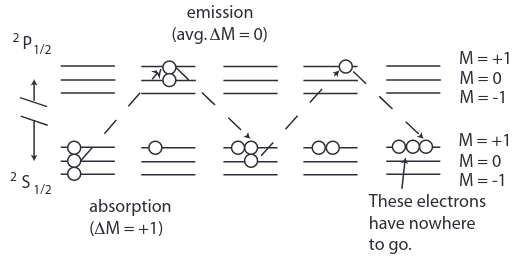
\includegraphics[scale= 0.5]{pictures/pumpen.png}
    \caption{Schematischer Vorgang des optischen Pumpens bei Wasserstoffatomen \cite{OpticalPumping}.}
    \label{fig:pumpen}
\end{figure}
\noindent
Zusätzlich zur spontanen Emission tritt auch die stimulierte Emission
auf, bei welcher ein Photon auf ein angeregtes Elektron tifft und 
eine Abregung dieses induziert. Dabei wird ein weiteres Photon 
frei, welches mit dem ersten Photon in Richtung, Polarisationsrichtung
und Phase übereinstimmt. Dieses Photon ist dementsprechend rechts zirkular
polarisiert. Somit ist $\Delta M_F=-1$. Dieser Effekt verzögert das 
optische Pumpen.

%Herunterspringen von dem gepumpten Niveau zu vernachlässigen, da wegen 
%$\propto f^3$ sehr unwahrscheinlich 

\noindent
Ein Maß für die Besetzungsinversion ist die Transparenz des 
Rubidiumgases. Ist die Besezung hoch können nur sehr wenige Photonen
Elektronen anregen. Ein Großteil der Photonen kann dann ungehindert
durch das Gas hindurch dringen, die Transparenz ist also hoch. 

\noindent
Durch ein weiteres, hochfrequentes, magnetisches Feld (RF-Feld) kann
die stimulierte Emission angeregt werden. Entspricht die duch das
RF-Feld gegebene Energie $E_{RF}=hf$ der Zeeman Energie $\Delta E_Z$
wird die Besetzungsinversion weitestgehend aufgehoben. Dies geschieht
bei einer magnetischen Flussdichte von
\begin{equation}
    B_m=\frac{hf}{g_F\mu_B} .
\end{equation}
Insbesodere ist als $B_m\propto f$. In Abbildung $\ref{fig:TB}$ ist 
die Transparenz als Funktion des Magnetfeldes aufgetragen.

\begin{figure}[H]
    \centering
    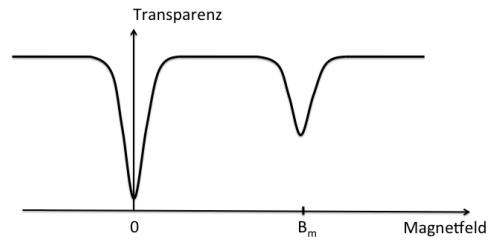
\includegraphics[scale= 0.5]{pictures/TB.png}
    \caption{Transparenz des Rb-Gases als Funktion des Magentfeldes \cite{V21}.}
    \label{fig:TB}
\end{figure}

\subsection{Magnetische Eigenschaften einer Helmholtz-Spule}
Eine Helmholtz Spule besteht aus zwei gleich großen, kreisförmigen 
Spulen mit Radius $R$, die parallel im Abstand $R$ angeodnet sind. 
Beide Spulen werden von dem gleichen Strom $I$ druchflossen. Zwischen 
den Spulen stellt sich ein homogenes Magnetfeld mit der Flussdichte
\begin{equation}
    B=\mu_0\frac{8IN}{\sqrt{125}R}
\end{equation}
ein. $N$ bezeichnet dabei die Windungszahl der Spule. 